% !TEX root=../index.tex

\chapter{Caratteristiche del Sensore Kinect} % (fold)
\label{chap:kinect}

Ciò che viene comunemente chiamato \emph{sensore di profondità} o \emph{sensore di distanza}, trova due differenti realizzazioni, a seconda della versione del Kinect.

\begin{figure}[h]
    \centering
    \begin{subfigure}[b]{0.48\textwidth}
    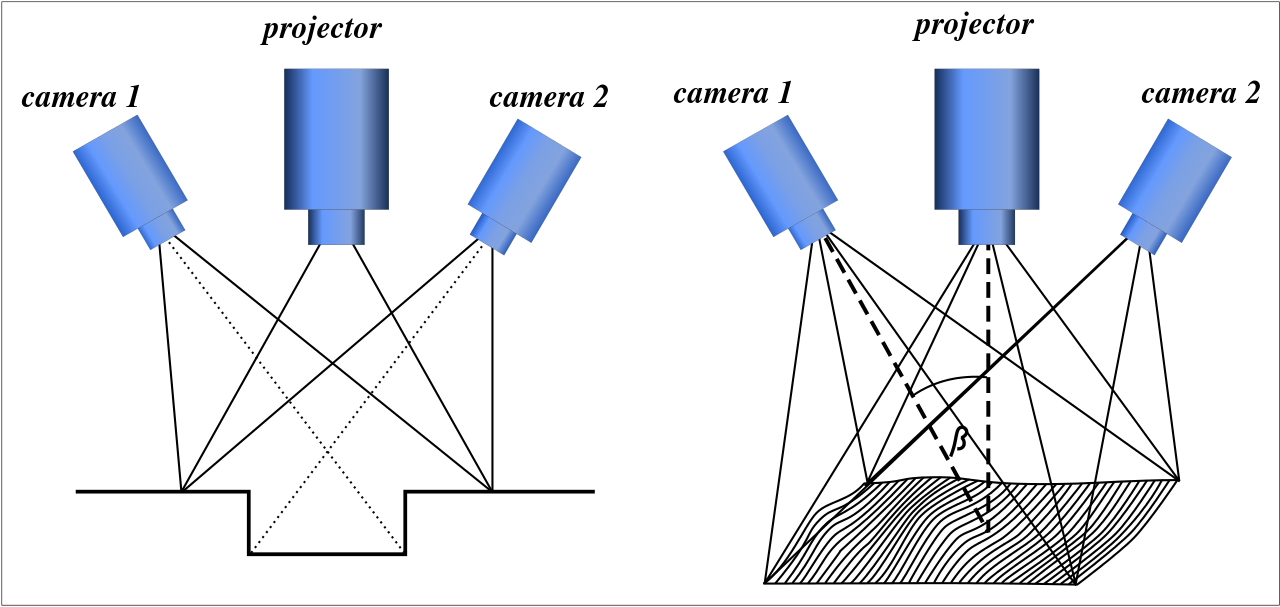
\includegraphics[width=\linewidth]{img/3d-structured-light-scanner.png}
        \caption{}
        \label{fig:3d_scanner}
    \end{subfigure}
    ~ %add desired spacing between images, e. g. ~, \quad, \qquad, \hfill etc. 
      %(or a blank line to force the subfigure onto a new line)
    \begin{subfigure}[b]{0.48\textwidth}
    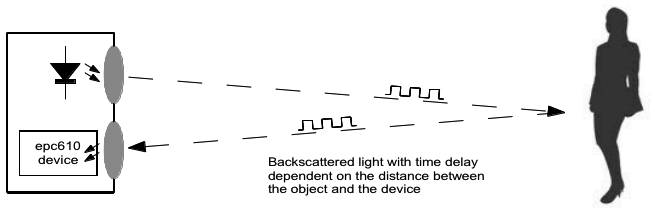
\includegraphics[width=\linewidth]{img/tof_camera.jpg}
        \caption{}
        \label{fig:tof_camera}
    \end{subfigure}
    \caption{Rappresentazione schematica di uno scanner a luce strutturata (\ref{fig:3d_scanner}) e di una \emph{TOF camera} (\ref{fig:tof_camera}).}
    \label{fig:distance_sensor}
\end{figure}

Il Kinect V1 utilizza uno \emph{scanner 3D a luce strutturata}, ovvero un dispositivo in cui una sorgente di raggi infrarossi proietta una serie di pattern codificati nello spazio.
Le superfici colpite inducono una deformazione nella struttura di tali pattern, che vengono quindi catturati da una o più telecamere, che confrontando la deformazione con il pattern originario.
Da questo confronto riescono a ricostruire, dalla rappresentazione bidimensionale di ogni punto nello spazio, le sue coordinate tridimensionali.

Il Kinect V2 invece utilizza una \emph{time of flight camera}: vengono inviati degli impulsi luminosi, quindi viene misurato il tempo che intercorre tra l'invio del segnale e la ricezione della radiazione di ritorno.
Dalla misura di questo intervallo (che altro non è che il tempo necessario alla luce per raggiungere l'oggetto e tornare indietro per il fenomeno della \emph{riflessione diffusa}) viene ricavata la distanza alla quale si trova il punto. 
Ripetendo questo procedimento si è in grado di costruire una rappresentazione tridimensionale dello spazio.

Il risultato di un sensore di questo tipo è un insieme di triplette $(x,y,z)$, organizzate in una \emph{immagine di profondità}, una struttura dati che è molto simile ad una semplice immagine in scala dei grigi\footnote{La forte somiglianza con le immagini in scala dei grigi è supportata dal fatto che ogni pixel è codificato utilizzando 16bit.}, dove il valore di ogni pixel rappresenta la misura in millimetri della distanza della superficie dal sensore.

La massima affidabilità del sensore del Kinect V2 si ha per distanza comprese tra $50cm$ e $4,5m$.
Il dispositivo è montato al soffitto a $2,8m$ da terra e ha un campo visivo di $70^{\circ} \times 60^{\circ}$, il quale, all'altezza del pavimento, determina un'area di cattura di circa $4m \times 5m$.

La dimensione di ogni immagine di profondità è di $512 \times 424$ pixel. 
Nativamente non vengono codificate in alcun modo particolare, sono delle semplici matrici di interi.
È in grado di catturarne fino a 30 al secondo. 
Utilizzando un apposito software di registrazione è stato possibile mettere insieme dei video di profondità a 30 fps.

% chapter kinect (end)